

\chapter{Multinomial methods for Variance Gamma}\label{Chapter3}
%\blindtext
\minitoc% Creating an actual minitoc

\vspace{5em}


 
In this chapter we make a digression about the application of a multinomial approximation for the Variance Gamma (VG) process.
The chapter collects the main results presented in the paper \cite{Canta2}. In Chapter \ref{Chapter6} this method is applied to solve the option pricing problem with 
transaction costs.\\
 
The VG process has nice analytical properties and 
reproduce quite well the statistical features of the financial data (see for instance \cite{Ait12} and \cite{Cont}).
In Figure \ref{FigPDF} we present as examples the histograms of the
daily log-returns for four of the major indices:  
the S\&P 500 Stock Index, 
the KOSPI (Korea Composite Stock Price Index), 
XAO (All Ordinaries Australian Index)  
and TAIEX (Taiwan Capitalization weighted Stock Index).
In the pictures we show the Normal and Variance Gamma (VG) densities fitted with the market data. 
It is straightforward to check that the 
VG density reproduces much better the high peaks near the origin, and the heavy tails feature.

\begin{figure}[t!]
 \centering
 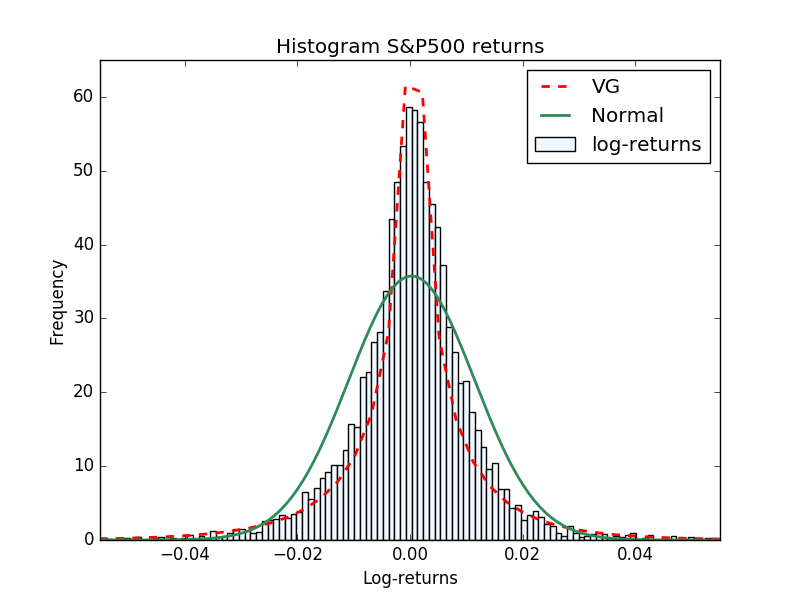
\includegraphics[width=0.47\textwidth]{sp500.png}
 ~
 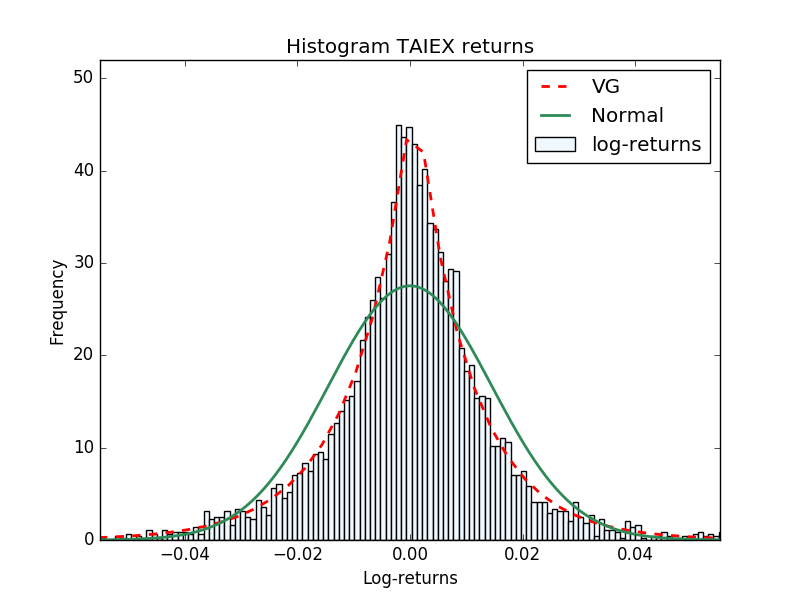
\includegraphics[width=0.47\textwidth]{twii.png}
 ~
 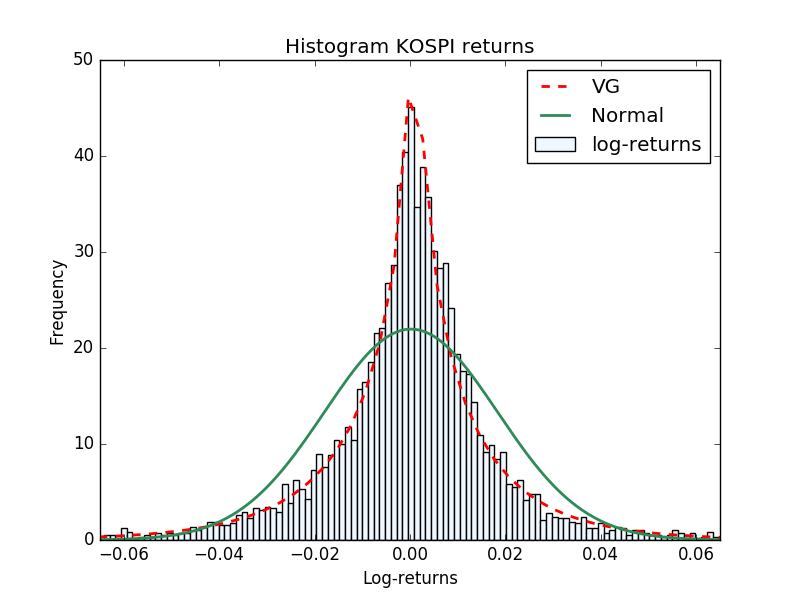
\includegraphics[width=0.47\textwidth]{kospi.png}
 ~
 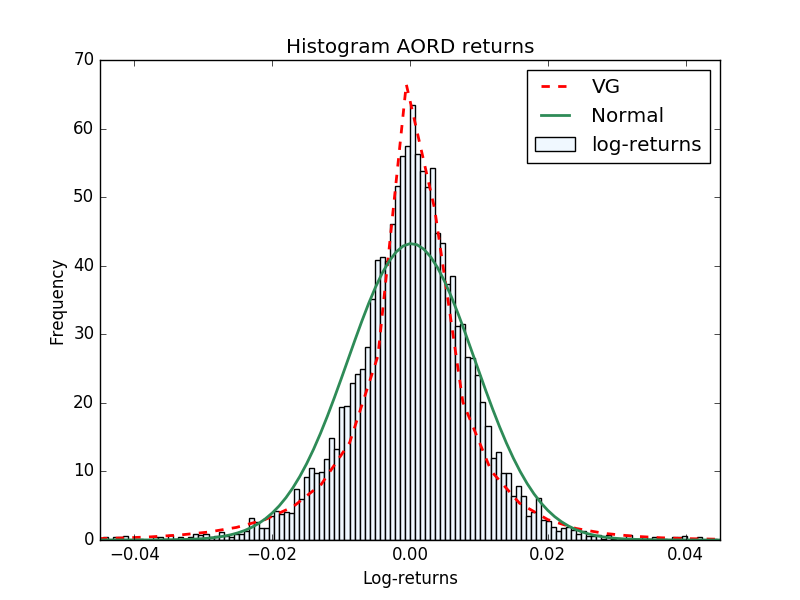
\includegraphics[width=0.47\textwidth]{xao.png}
 % VG4_pdf.png: 0x0 pixel, 0dpi, 0.00x0.00 cm, bb=
 \caption{Histograms of daily log-returns for S\&P500, KOSPI, XAO and TAIEX. The dashed line corresponds to the VG density (\ref{VG_density}). 
 The continuous line is the normal density. The parameters for both densities are obtained by the \emph{method of moments} (details in \cite{Se04}).}
 \label{FigPDF}
\end{figure} 

The VG process was first presented in the context of option pricing 
in \cite{MaMi91}, where it has been used for pricing European options.
European vanilla options can be easily priced by the analytical formula presented in \cite{MCC98} and exotics
can be priced numerically by several techniques:
Monte Carlo methods for VG are presented in \cite{Fu00}. 
A finite difference scheme for the VG Partial Integro-Differential Equation (PIDE) 
is described in \cite{CoVo05b}. In \cite{CaMa98}, the authors show how to price options by using a Fourier transform approach.
The problem for American options is considered in \cite{Al05}, \cite{Oo05} and \cite{HiMa01}, where the authors present different finite difference 
schemes to solve the American VG PIDE.

The tree method was first introduced by \cite{CRR79} for a market where the log-price can change only in two different ways: 
an upward jump, or a downward jump. For this reason the model is called \emph{binomial model}. The authors 
prove that when the number of time steps goes to infinity, the discrete random walk of the log-price converges to the Brownian motion
and the option price converges to the Black-Scholes price.
The \emph{multinomial model} is a generalization of the binomial model, and at each time step it considers 
more than just two possible future states.
A general multinomial method for pricing European and American options under exponential L\'evy processes is described in \cite{MaSoSz}. 
In \cite{KeWe06} the authors consider a multinomial method for general exponential L\'evy processes based on the moment matching condition.
Other methods based on the moment matching condition are for instance \cite{HaMac10}, with applications to the Normal Inverse Gaussian process, and 
\cite{See13} with applications to the VG process.  
In the present work we consider a multinomial discretization based on the cumulant matching condition as explained in \cite{YaPr01}, \cite{YaPr03} and \cite{YaPr06}. 


In Section \ref{sec3_ch3} we review the construction of the multinomial tree, following the method of
moment matching proposed in \cite{YaPr01}. We prove that the multinomial tree converges to the continuous time jump process that we have
introduced to approximate the VG process.
In Section \ref{sec4_ch3}, which is the most important of the paper, we describe the algorithm for pricing options with the 
multinomial method and show the numerical results for European and American options.




\section{The multinomial method} \label{sec3_ch3}
In this section we introduce the multinomial method proposed in \cite{YaPr06}. 
The stock price is considered as a Markov chain with $L$ possible future states at each time. 
In this setting, the time $t \in [t_0,T]$ is discretized as $t_n = t_0 + n\Delta t$ for $n=0, ... ,N$ and 
$\Delta t = (T-t_0)/N$. We denote the stock price at time $t_n$ as $S(t_n) = S_n$.

Consider the up/down factors $u>d>0$ and write the discrete evolution of the stock price $S_n$ as:
\begin{equation}\label{Discr_S}
  S_{n+1} = u^{L-l}d^{l-1} S_n  \hspace{3em} l=1, ... , L  
\end{equation}
where each future state has transition probability $p_l$, satisfying $\sum_{l=1}^L p_l = 1$.
The value of the stock at time $t_n$ can assume $j \in [1,...,n(L-1)+1]$ possible values:
\begin{equation}\label{Discr_S2}
  S_{n}^{(j)} = u^{n(L-l)+1-j}d^{j-1} S_0.  
\end{equation}
The multinomial tree is recombining if for a constant $c>1$, $u/d = c$.
Regarding the present work, we only consider five branches, $L=5$. As explained in \cite{YaPr06}, this number of branches is 
enough to model the features of a stochastic process up to its fourth moment.


\subsection{Moment matching}

To determine the parameters of the Markov chain we require that its local moments are equal to that of the continuous process.
First, we rewrite the continuous process (\ref{VG_sde}) using the log-variable $Y_t = \log(S_t)$ (as explained in Section \ref{VG_section2}) 
obtaining:
\begin{align}\label{log_martingale}
 Y_{t+\Delta t}-Y_t &= (r+\omega)\Delta t + \int_{\R} x N(\Delta t,dx) \\ \nonumber
		    &= (r+\omega + \theta)\Delta t + \int_{\R} x \tilde N(\Delta t,dx)
\end{align}
where $\theta = \int_{\R} x \nu(dx) = \E \bigl[ \int_{\R} x N(1,dx) \bigr]$ is the expected value of the VG process in (\ref{VG_process}), 
when $\Delta t=1$. 
The integral with respect to the compensated Poisson measure $\tilde N(\Delta t,dx)$ is a martingale as discussed in Section \ref{random_measures}.

We can pass to log-prices $Y_n = \log(S_n)$ in the discrete Eq. (\ref{Discr_S}), and write it as the sum of a drift component and a 
random variable with $L$ possible outcomes:
\begin{align}\label{Discr_Y}
 \Delta Y = Y_{n+1} - Y_n &= (L-l) \log(u) + (l-1) \log(d) \\ \nonumber
  &= \bar b\, \Delta t + (L-2l+1) \alpha(\Delta t).
\end{align}
The term $\bar b\, \Delta t$ is the drift term, while $l$ is a random variable that assumes values in $\{1,2,...,L\}$ with probability $p_l$. 
It has to satisfy the martingale condition:
$$ \E \bigl[(L-2l+1) \alpha(\Delta t) \bigr] = \alpha(\Delta t) \sum_{l=1}^L p_l (L-2l+1) = 0, $$
with $\alpha(\Delta t)$ a function of $\Delta t$.

The corresponding up/down factors have the following representation:
\begin{equation}\label{updown}
 u = \exp\biggl( \frac{b}{L-1} + \alpha(\Delta t) \biggr) \hspace{2em}  d = \exp\biggl( \frac{b}{L-1} - \alpha(\Delta t) \biggr),
\end{equation}
and we can readily see that if $u/d$ is constant the tree recombines.

Given the mean $c_1 = \E[\Delta Y] = \bar b \Delta t$, the $k$-central moment is:
\begin{equation}\label{higher_moments}
 \E \bigl[ (\Delta Y - c_1)^k \bigr] = \alpha(\Delta t)^k\, \E \bigl[ (L-2l+1)^{k} \bigr].
\end{equation}
The moment matching condition requires that the central moments of the discrete process (\ref{Discr_Y}) 
are equal to the central moments
of the continuous process (\ref{log_martingale}):
\begin{equation}\label{moment_matching}
 \alpha(\Delta t)^k\, \E \bigl[ (L-2l+1)^{k} \bigr] = \mu_k.
\end{equation}
We fix $L=5$, and using the relation between central moments and cumulants (Eq. (\ref{moment_cumulants}) )
we solve the linear system of equations for the transition probabilities:
\begin{align}\label{probabilities1}
 p_1 &= \frac{1}{196 \alpha(t)^4} \biggl[ \frac{3}{2} c_2^2 -2 c_2\alpha(t)^2 + 2 c_3 \alpha(t) +\frac{1}{2} c_4  \biggr] \\ \nonumber
 p_2 &= \frac{1}{196 \alpha(t)^4} \biggl[ -6 c_2 + 32c_2 \alpha(t)^2 - 4c_3 \alpha(t) -2 c_4 \biggr] \\ \nonumber
 p_3 &=  1 + \frac{1}{196 \alpha(t)^4} \biggl[ 3c_4 + 9c_2^2 -60c_2 \alpha(t)^2   \biggr] \\ \nonumber
 p_4 &= \frac{1}{196 \alpha(t)^4} \biggl[ -6 c_2 + 32c_2 \alpha(t)^2 + 4c_3 \alpha(t) -2 c_4  \biggr] \\ \nonumber
 p_5 &= \frac{1}{196 \alpha(t)^4} \biggl[ \frac{3}{2} c_2^2 -2 c_2\alpha(t)^2 - 2 c_3 \alpha(t) +\frac{1}{2} c_4 \biggr].
\end{align}
The drift parameter corresponds to $\bar b = r+\omega + \theta$.
The only missing parameter to determine is $\alpha(\Delta t)$. This is a function of the time increment $\Delta t$ and can be determined using the 
higher order terms in the moment matching condition together with the condition of positive probabilities.

Recall that the well known binomial model \cite{CRR79} assumes the value $\alpha(\Delta t) = \sigma \sqrt{\Delta t}$,
that represents the volatility of the increments in the time interval $\Delta t$.
In the trinomial model, the parameter $\alpha(\Delta t)$ assumes value $\alpha(\Delta t) = \frac{1}{2} \sigma \sqrt{3\Delta t}$, see for instance \cite{YaPr01}.
For the multinomial method a good representation for $\alpha(\Delta t)$ is:
\begin{equation}\label{alphat}
 \alpha(\Delta t) = \sqrt{c_2} \sqrt{\frac{3+\bar \kappa}{12}},
\end{equation}
where $\bar \kappa = c_4 / c_2^2$ is the excess of kurtosis\footnote{We use the bar over $\kappa$, 
to distinguish the kurtosis from the variance of the gamma process $\kappa$.}. 
We refer to \cite{YaPr06} for the derivation.
This choice guarantees that the probabilities $p_i$ for $i=1...5$ are always positive and sum to one. We can replace the expression
(\ref{alphat}) inside (\ref{probabilities1}), to obtain the simpler form:
\begin{align}\label{probabilities2}
 & [p_1,p_2,p_3,p_4,p_5] \approx \biggl[ \frac{3+\bar \kappa+s\sqrt{9+3\bar \kappa}}{4(3+\bar \kappa)^2} , 
 \frac{3+\bar \kappa-s\sqrt{9+3\bar \kappa}}{2(3+\bar \kappa)^2} , \\ \nonumber
 &
 \frac{3+2\bar \kappa}{2(3+\bar \kappa)} ,
 \frac{3+\bar \kappa+s\sqrt{9+3\bar \kappa}}{2(3+\bar \kappa)^2} ,
 \frac{3+\bar \kappa-s\sqrt{9+3\bar \kappa}}{4(3+\bar \kappa)^2} \biggr],
\end{align}
where $s = c_3 / \sqrt{c_2^3}$ is the skewness.
\begin{Remark}
 The standard deviation of every L\'{e}vy process with finite moments follows the square root propagation rule. This means that the term $\alpha(\Delta t)$ has to be proportional
 to the square root of $\Delta t$. In the binomial and trinomial models, the proportionality constant is explicit, while for the pentanomial method it is implicit
 in the formula (\ref{alphat}). Expanding the formula using the expression (\ref{VG_cumulants}) for the cumulants, it is possible to check that the square root rule is
 satisfied at first order in $\sqrt{\Delta t}$.
\end{Remark}



\subsection{Convergence}


We call a generic jump process (\ref{Levy_Ito3}) with first four cumulants $c_1$,$c_2$,$c_3$,$c_4$ as in (\ref{VG_cumulants}), 
the \emph{approximated process} $X^A$. 
The cumulant generating function of the increment $\Delta X^A$ has the following series representation (see Section \ref{cumulant_sec} ):
\begin{equation}\label{cum_gen_appr}
 H_{\Delta X^{A}}(u) = ic_1 u -\frac{c_2u^2}{2} -\frac{ic_3u^3}{3!} + \frac{c_4u^4}{4!} + \mathcal{O}(u^5).
\end{equation}
We are interested in the approximation of a VG process with drift (\ref{log_martingale}), therefore we require that $c_1 = \bar b \Delta t = (r+\omega+\theta)\Delta t$. 
\begin{Theorem}
The increments of the discrete Markov chain (\ref{Discr_Y}) and the increments of the approximated process $X^A$ have the same distribution by construction.
\end{Theorem}
\begin{proof}
The idea of the proof is to show that the cumulant generating function of the discrete process (\ref{Discr_Y}) 
coincides with that of the approximated process (\ref{cum_gen_appr}). We prove it using the moment
matching condition (\ref{moment_matching}).
\begin{align}
H_{\Delta Y}(u) &= \log \bigl( \phi_{\Delta Y}(u)  \bigr) = \log \biggl( \E \bigl[ e^{iu \Delta Y} \bigr] \biggr) \\ \nonumber
                &= \log \biggl( \E \biggl[ e^{iu \bigl( \bar b \Delta t + (L-2l+1) \alpha(\Delta t) \bigr) } \biggr] \biggr) \\ \nonumber
		&= iu \bar b \Delta t + \log \biggl( \E \biggl[ e^{iu \bigl(  (L-2l+1) \alpha(\Delta t) \bigr) } \biggr] \biggr).
\end{align}
We can expand the exponential function in Taylor series and use the moment matching condition (\ref{moment_matching}) to obtain:
\begin{align}
H_{\Delta Y}(u) &= iu \bar b \Delta t + \log \biggl( \sum_{k=0}^{\infty} \frac{(iu)^k}{k!} 
\bigl(\alpha(\Delta t)\bigr)^k \E \biggl[ \bigl( L-2l+1  \bigr)^k \biggr] \biggr) \\ \nonumber
                &= iu \bar b \Delta t + \log \biggl( \sum_{k=0}^{\infty} \frac{(iu)^k}{k!} \mu_k \biggr) \\ \nonumber
                &= iu c_1 + \sum_{k=0}^{\infty} \frac{(iu)^k}{k!} c_k \\ \nonumber 
                &= H_{\Delta X^{A}}(u),
\end{align}
\end{proof}
\begin{Remark}
All the cumulants of $\Delta X^A$ are equal to the cumulants of the Markov chain (\ref{Discr_Y}) by construction, but only the first four are equal to the VG cumulants.
When all the cumulants $c_i$, for $0 \leq i \leq n$, are equal to the VG cumulants, the approximated process $X^A$ converges to
the original VG process for $n \to \infty$.
To control $n$ cumulants, we need $n+1$ branches. Therefore, when the number of cumulants of $\Delta X^A$ equal to those of the VG process goes to infinity, 
the number of branches have to go to infinity as well.
We assume that five branches ($L=5$) are enough to describe the features of the underlying process and, at the same time, keep the numerical
problem simple. 
\end{Remark}

\begin{Theorem}
The distribution of the pentanomial tree at time $N$ converges to the distribution of a compound Poisson process at time $N$ with $L=5$ possible jump sizes and activity $\lambda = \frac{3}{2 \bar \kappa N}$, when $\Delta t \to 0$.   
\end{Theorem}
For the proof of this theorem  
we refer to Section 4.2 of \cite{YaPr06}. The authors first define the jump sizes and their respective probabilities, and then
prove that when $\Delta t \to 0$ the characteristic function of the pentanomial tree converges to the 
characteristic function of the compound Poisson process.



\section{Numerical results} \label{sec4_ch3}

In this section we present the steps to implement the algorithm for pricing European and American options with the multinomial method.
Then we compare the results with those obtained by the PIDE method and Black-Scholes model.

\subsection{Algorithm}

We suggest the following algorithm for pricing with the multinomial method:
\begin{enumerate}
 \item Compute the transition probabilities vector (\ref{probabilities2}). 
 \item Compute the up/down factors $u$ and $d$ (\ref{updown}) and the vector of prices $S_N$ at terminal time $N$ as in Eq. (\ref{Discr_S2}).
 \item Evaluate the payoff of the option $V^N(S_N)$ at terminal time $N$.
 \item Given the option's values at time $t_{n+1}$ compute the values at time $t_n$. The value is the conditional expectation:
 \begin{equation}
 V^n(s^{(k)}_n) = e^{-r\Delta t} \E^{\Q} \biggl[ V^{n+1}(S_{n+1}) \bigg| S^{(k)}_n = s^{(k)}_n \biggr]. 
\end{equation}
 \item If computing the price of an American option, the value at the previous time level is the maximum between the conditional expectation and
 the intrinsic value of the option. For an American put we have:
 \begin{equation}
 V^n(s^{(k)}_n) = \max \biggr \{ e^{-r\Delta t} \E^{\Q} \biggl[ V^{n+1}(S_{n+1}) \bigg| S^{(k)}_n = s^{(k)}_n \biggr] , K-s^{(k)}_n \biggr \}. 
\end{equation}	
 \item Iterate the algorithm until the initial time $t_0$. 
\end{enumerate}
In the parameters calibration procedure, sometimes it is common to estimate first the historical parameters, and use them as initial guess for the
least squares minimization that recovers the risk neutral parameters.
In \cite{Se04} are presented several methods for historical parameters estimation of the VG density. We use the simple method of moments to estimate the 
parameters for the data in Fig. \ref{FigPDF}.
In all future calculations we consider the risk neutral VG parameters in Table \ref{sample-table}.

\begin{table}[!h]
\centering
{\begin{tabular}{llll}
\toprule
 \multicolumn{4}{c}{Parameters} \\
\midrule
$r$ & $\theta$ & $\sigma$ & $\kappa$ \\ 
0.06 & -0.1 & 0.2 & 0.2 \\
\bottomrule
\end{tabular}}
\caption{$r$ is the risk free interest rate and $\theta, \sigma, \kappa$ are the risk neutral VG parameters.}
\label{sample-table}
\end{table}



\subsection{European options}


We compare the numerical results for European call and put options obtained with the multinomial and the PIDE approaches.
\begin{itemize}
 \item \emph{VG PIDE}: We solve the VG PIDE following the method proposed in section \ref{VG_section2}.
 We solve the PIDE (\ref{VG_JD}) using the implicit-explicit finite difference scheme, and choosing the truncator parameter $\epsilon = 1.5 \delta x$, 
 where $\delta x$ is the size of 
 the space step. It turns out that the solution of the discretized equation convergences very slowly to the option price, and therefore we required a grid with $14000$ space steps 
 and $7000$ time steps. The algorithm is written in Matlab and runs
 on an Intel i7 (7th Gen) with Linux. It takes about 30 minutes to complete. 
 \item \emph{Multinomial}: We follow the algorithm proposed in the previous section. The number of time steps for all the computations is $N=2000$. In the table \ref{Convergence} 
 we show a convergence table for the prices of European calls, puts and American puts. It is straightforward to see that the convergence is quite fast.  
\end{itemize}
\begin{table}[ht]
\centering
{\begin{tabular}{llllll}
\toprule
  $N$ & Eu. Call & Eu. Put & Time & Am. Put & Time \\
\midrule
    50 & 4.41873125 & 2.08928091 & 0.001 & 2.36765911 & 0.007 \\
    100 & 4.41960265 & 2.09015381 & 0.002 & 2.37255454 & 0.02 \\
    200 & 4.41997010 & 2.09052201 & 0.004 & 2.37480218 & 0.07 \\
    400 & 4.42013640 & 2.09068869 & 0.01 & 2.37587117 & 0.29 \\
    800 & 4.42021515 & 2.09076762 & 0.03 & 2.37639131 & 1.09 \\
    1000 & 4.42023054 & 2.09078306 & 0.04 & 2.37649417 & 1.67 \\
    1500 & 4.42025089 & 2.09080345 & 0.06 & 2.37663070 & 3.79 \\
    2000 & 4.42026098 & 2.09081357 & 0.10 & 2.37669869 & 6.80 \\
    2500 & 4.42026701 & 2.09081962 & 0.16 & 2.37673941 & 10.65 \\
    3000 & 4.42027102 & 2.09082364 & 0.2 & 2.37676652 & 14.78 \\
  \bottomrule
\end{tabular}}
\caption{Convergence table for ATM European and American options with strike $K=40$ and $T=1$. The time unit is in seconds.}
\label{Convergence}
\end{table}
Figures (\ref{figCall}) and (\ref{figPut}) show the prices obtained by the multinomial method compared with those obtained by PIDE.
In table \ref{Option_values} we compare directly the call/put numerical values obtained with the two methods.
\begin{figure}[t!]
 \begin{minipage}[b]{0.5\linewidth}
   \centering
 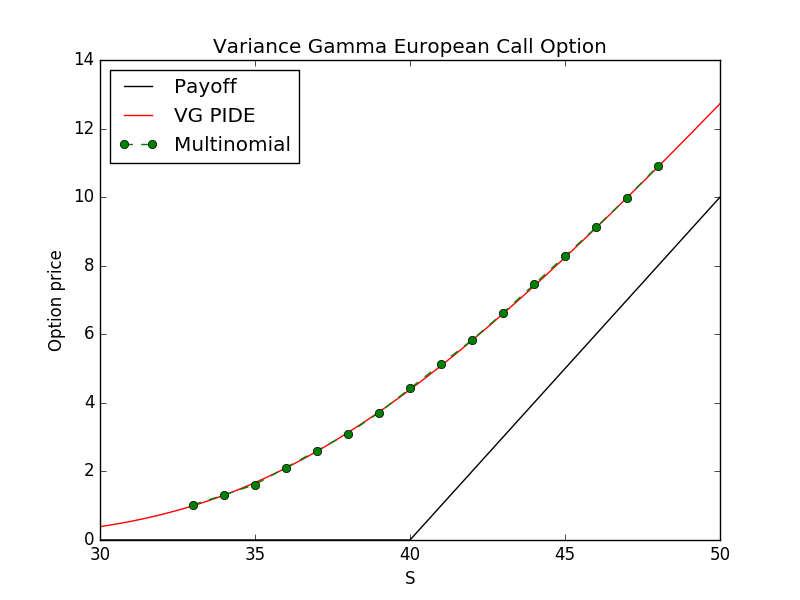
\includegraphics[width=\linewidth]{EU_call.png}
 % EU_call.png: 0x0 pixel, 300dpi, 0.00x0.00 cm, bb=
 \caption{European call option with strike $K=40$ and time to maturity 1 year.}
 \label{figCall}
  \end{minipage}
 \ \hspace{2mm} \hspace{3mm} \
 \begin{minipage}[b]{0.5\linewidth}
 \centering
 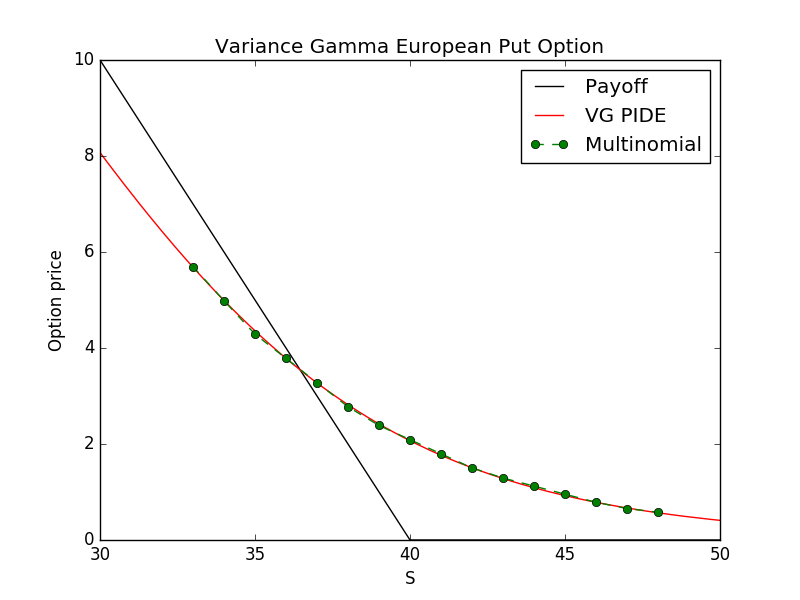
\includegraphics[width=\linewidth]{EU_put.png}
 % EU_call.png: 0x0 pixel, 300dpi, 0.00x0.00 cm, bb=
 \caption{European put option with strike $K=40$ and time to maturity 1 year.}
 \label{figPut}
 \end{minipage}
\end{figure}

Pricing vanilla call and put European options is quite simple and the best approach is to use the closed formula derived in \cite{MCC98}.
The big advantage of the multinomial method is in the computation of American options prices, where there is no closed formula and all the other approaches, 
such as PIDEs and Least Squares Monte Carlo, are difficult to implement and much slower.
\begin{table}[ht]
\centering
{\begin{tabular}{lllll} 
\toprule
\multicolumn{5}{c}{Different methods} \\
\midrule
$S_0$ & PIDE Call & Multi Call & PIDE Put & Multi Put \\
\midrule
36 & 2.1036 & 2.1131 & 3.7842 & 3.7837  \\
  38 & 3.1163 & 3.1051 & 2.7893 & 2.7756 \\
  40 & 4.4162 & 4.4203 & 2.0852 & 2.0908 \\
  42 & 5.8335 & 5.8309 & 1.5050 & 1.5014 \\
  44 & 7.4417 & 7.4524 & 1.1132 & 1.1229 \\
\bottomrule
\end{tabular}}
\caption{European Options, with strike $K=40$ and $T=1$.}
\label{Option_values}
\end{table}



\subsection{American options}

In this section we present the numerical results obtained with the multinomial method algorithm for American put options, and compare them with the PIDE method (see fig. \ref{AmVG}).
The PIDE (\ref{VG_JD}) is modified in order to take in account the early exercise feature:
\begin{align}\label{VG_Am_JD}
&  \min \biggl\{ - \frac{\partial V(t,x)}{\partial t} -
 \bigl( r-\frac{1}{2}\sigma_{\epsilon}^2 - w_{\epsilon} \bigr) \frac{\partial V(t,x)}{\partial x} 
 - \frac{1}{2}\sigma_{\epsilon}^2 \frac{\partial^2 V(t,x)}{\partial x^2} + (\lambda_{\epsilon} + r) V(t,x) \\ \nonumber
 &- \int_{|z| \geq \epsilon} V(t,x+z) \nu(dz) \, , \, \biggl( V(t,x) - (K-e^x)^+ \biggr) \biggr\} = 0.
\end{align}
To solve this equation we use the same settings used for the Eq. (\ref{VG_JD}): an implicit-explicit finite difference scheme, with 14000 space steps and 7000 time steps. 
The algorithm takes about 33 minutes to run.

The numerical values of the prices obtained with the multinomial and PIDE methods are collected in Tab. \ref{Option_values3}.
The run times for the multinomial algorithm are shown in the convergence table \ref{Convergence}.
\begin{figure}[ht!]
 \centering
 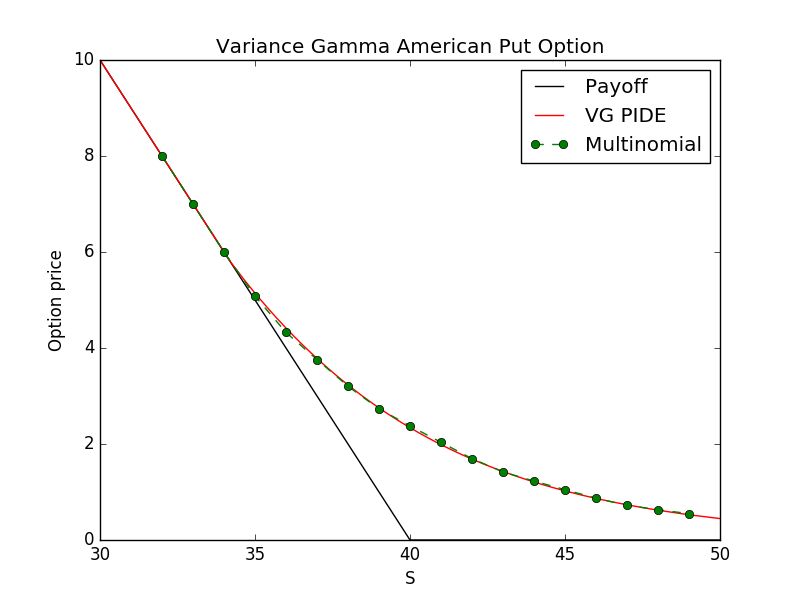
\includegraphics[scale=0.4]{American_VG.png}
 % EU_call.png: 0x0 pixel, 300dpi, 0.00x0.00 cm, bb=
 \caption{American put option with strike $K=40$ and time to maturity 1 year. Comparison of PIDE prices and multinomial prices.}
 \label{AmVG}
\end{figure}
\begin{table}[ht]
{\begin{tabular}{llllll}
\toprule
 \multicolumn{6}{c}{Prices comparison} \\
\midrule
$S_0$ & BS Eu. Put & VG Eu. Put & BS Am. Put & VG Am. Put & VG Am. PIDE Put \\
 \midrule
  30 & 8.1316 & 8.0809 & 10     & 10     & 10 \\
  32 & 6.5292 & 6.4055 & 8      & 8      & 8 \\
  34 & 5.1169 & 4.9851 & 6.0894 & 6      & 6 \\
  36 & 3.9150 & 3.7837 & 4.5415 & 4.3173 & 4.3982 \\
  38 & 2.9263 & 2.7756 & 3.3264 & 3.2034 & 3.2195 \\
  40 & 2.1388 & 2.0908 & 2.3924 & 2.3767 & 2.3531 \\
  42 & 1.5322 & 1.5014 & 1.6911 & 1.6947 & 1.6849 \\
  44 & 1.0766 & 1.1229 & 1.1755 & 1.2267 & 1.2118 \\
  46 & 0.7433 & 0.7858 & 0.8043 & 0.8699 & 0.8650 \\
  48 & 0.5049 & 0.5787 & 0.5425 & 0.6310 & 0.6221 \\
  50 & 0.3384 & 0.4259 & 0.3612 & 0.4661 & 0.4480 \\ 
  52 & 0.2238 & 0.3015 & 0.2376 & 0.3242 & 0.3222 \\
  55 & 0.1178 & 0.1909 & 0.1243 & 0.2051 & 0.1990 \\
  60 & 0.0386 & 0.0880 & 0.0404 & 0.0942 & 0.0913 \\ 
 \bottomrule
 \end{tabular}}
  \label{Option_values3}
  \caption{Values for European and American put options using Black-Scholes and Variance Gamma model. Strike $K=40$ and $T=1$. The BS volatility have same value of the VG volatility:  
  $ \sigma^{BS} = (\sigma^2 + \theta^2 \kappa) = 0.2049$. }
\end{table}

In Table \ref{Option_values3}, we consider also European and American put option prices 
calculated with the Black-Scholes (BS) models.
The BS volatility is chosen equal to the VG volatility $ \sigma^{BS} = (\sigma^2 + \theta^2 \kappa)$.
As expected, the deep OTM (out of the money) prices computed under VG are higher than the corresponding prices computed under BS. This is a consequence of the
shape of the VG density function (\ref{VG_density}), which has \emph{heavier tails} than the normal distribution. This means that the probability of a deep OTM option to return in the money, 
is higher if calculated with the VG model than BS, and therefore we get higher option prices.

The Black-Scholes prices are computed using a binomial algorithm. For European options the prices converge to the BS closed formula prices. 
The same values can be obtained using the multinomial algorithm for the VG process and setting $\theta = \kappa = 0$ and $\sigma = \sigma^{BS}$.
Recall that under the Black-Scholes model, the log-returns follow a Brownian motion. 
Looking at the definition of the VG process (\ref{VG_process}), it is evident that when $\theta$ and $\kappa$ are zero, the process becomes a Brownian motion:
$$ X^{VG}_t \underset{\theta,\kappa \to 0}{\to} \sigma W_t. $$
As a consequence, the price process converges to the Geometric Brownian Motion:
$$ S_t = S_0 e^{(r+\omega)t + X_t} \underset{\theta,\kappa \to 0}{\to} S_0 e^{(r-\frac{1}{2}\sigma^2)t + \sigma W_t} $$
where:
\begin{align*}
 \lim_{\theta,\kappa \to 0} w &= \lim_{\theta,\kappa \to 0} \frac{1}{\kappa} \log(1-\theta \kappa -\frac{1}{2}\sigma^2 \kappa) \\
 &= -\frac{1}{2}\sigma^2.
\end{align*}


